\documentclass{report}

% Language setting
% Replace `english' with e.g. `spanish' to change the document language
\usepackage[english]{babel}
\usepackage{blindtext}
\usepackage{titlesec}

% Useful packages
\usepackage{amsmath} % math alignment
\usepackage{siunitx} % SI units
\sisetup{output-decimal-marker={,}} % make it so that \num uses commas for decimals
\sisetup{per-mode=symbol} % by default \per is set to power, fraction also works
\sisetup{power-half-as-sqrt} % literally what it says, sqrt instead of ^(0,5)
\usepackage{float}
\usepackage{caption}
\usepackage[skip=0.5ex]{subcaption} % using both subfigure and subcaption causes conflicts
%\usepackage{subfigure}
\usepackage{graphicx}

% float images to top with no whitespace 
\makeatletter
\setlength{\@fptop}{0pt}
\makeatother


\usepackage{xcolor}
\usepackage[
colorlinks=true,
urlcolor=blue,
linkcolor=., % red for drafts, set to . (same as surrounding text) otherwise
citecolor=., 
pdftitle={ComVis V.S. 26/27}
]{hyperref}
%\usepackage{cleveref} % better refs, always load after hyperref
\usepackage[toc]{appendix}
\usepackage{markdown}
\usepackage[table,xcdraw]{xcolor}
\usepackage{adjustbox}
\usepackage{braket} % package for ket (quantum) brackets
\usepackage{csquotes} % quotes using \say{}
\usepackage{matlab-prettifier}
\usepackage{wrapfig} % use for wrapping figures/tables
%\usepackage[all]{nowidow} % remove widows/orhans

% floats will not be placed in different subsections (control sequence is used for setting the float limit to subsections instead of sections)
\usepackage{placeins} 
\makeatletter
\AtBeginDocument{%
	\expandafter\renewcommand\expandafter\subsection\expandafter
	{\expandafter\@fb@secFB\subsection}%
	\newcommand\@fb@secFB{\FloatBarrier
		\gdef\@fb@afterHHook{\@fb@topbarrier \gdef\@fb@afterHHook{}}}%
	\g@addto@macro\@afterheading{\@fb@afterHHook}%
	\gdef\@fb@afterHHook{}%
}
\makeatother

% Set page size and margins
% Replace `letterpaper' with `a4paper' for UK/EU standard size
\usepackage[a4paper,top=2cm,bottom=2cm,left=3cm,right=3cm,marginparwidth=1.75cm]{geometry}

\usepackage{circuitikz} % drawing circuits
\usepackage{tikz, pgfplots} % drawing diagrams
\usetikzlibrary{positioning} % for positioning tikz elements (e.g. right=of, left=of)
\usetikzlibrary{backgrounds} % for drawing in the background (using scope environment)
\usetikzlibrary{decorations.pathreplacing} % for drawing curly braces with tikz

% Code listings
\usepackage{listings}
\colorlet{punct}{red!60!black}
\definecolor{background}{HTML}{EEEEEE}
\definecolor{delim}{RGB}{20,105,176}
\colorlet{numb}{magenta!60!black}

\usepackage{listings}
\lstset{basicstyle=\ttfamily}
\lstset{breaklines=true}

\lstdefinelanguage{json}{
	basicstyle=\normalfont\ttfamily,
	numbers=left,
	numberstyle=\scriptsize,
	stepnumber=1,
	numbersep=8pt,
	showstringspaces=false,
	breaklines=true,
	frame=lines,
	backgroundcolor=\color{background},
	literate=
	*{0}{{{\color{numb}0}}}{1}
	{1}{{{\color{numb}1}}}{1}
	{2}{{{\color{numb}2}}}{1}
	{3}{{{\color{numb}3}}}{1}
	{4}{{{\color{numb}4}}}{1}
	{5}{{{\color{numb}5}}}{1}
	{6}{{{\color{numb}6}}}{1}
	{7}{{{\color{numb}7}}}{1}
	{8}{{{\color{numb}8}}}{1}
	{9}{{{\color{numb}9}}}{1}
	{:}{{{\color{punct}{:}}}}{1}
	{,}{{{\color{punct}{,}}}}{1}
	{\{}{{{\color{delim}{\{}}}}{1}
	{\}}{{{\color{delim}{\}}}}}{1}
	{[}{{{\color{delim}{[}}}}{1}
	{]}{{{\color{delim}{]}}}}{1},
	morestring=[b]",
}

\lstdefinelanguage{curl}{
	basicstyle=\normalfont\ttfamily,
	numbers=left,
	numberstyle=\scriptsize,
	stepnumber=1,
	numbersep=8pt,
	showstringspaces=false,
	breaklines=true,
	frame=lines,
	backgroundcolor=\color{background},
	literate=
	*{0}{{{\color{numb}0}}}{1}
	{1}{{{\color{numb}1}}}{1}
	{2}{{{\color{numb}2}}}{1}
	{3}{{{\color{numb}3}}}{1}
	{4}{{{\color{numb}4}}}{1}
	{5}{{{\color{numb}5}}}{1}
	{6}{{{\color{numb}6}}}{1}
	{7}{{{\color{numb}7}}}{1}
	{8}{{{\color{numb}8}}}{1}
	{9}{{{\color{numb}9}}}{1}
	{:}{{{\color{punct}{:}}}}{1}
	{,}{{{\color{punct}{,}}}}{1}
	{\{}{{{\color{delim}{\{}}}}{1}
	{\}}{{{\color{delim}{\}}}}}{1}
	{[}{{{\color{delim}{[}}}}{1}
	{]}{{{\color{delim}{]}}}}{1},
	morestring=[b]",
}


\lstdefinelanguage{ino}{
	basicstyle=\normalfont\ttfamily,
	numbers=left,
	numberstyle=\scriptsize,
	stepnumber=1,
	numbersep=8pt,
	showstringspaces=false,
	breaklines=true,
	frame=lines,
	backgroundcolor=\color{background},
	literate=
	*{0}{{{\color{numb}0}}}{1}
	{1}{{{\color{numb}1}}}{1}
	{2}{{{\color{numb}2}}}{1}
	{3}{{{\color{numb}3}}}{1}
	{4}{{{\color{numb}4}}}{1}
	{5}{{{\color{numb}5}}}{1}
	{6}{{{\color{numb}6}}}{1}
	{7}{{{\color{numb}7}}}{1}
	{8}{{{\color{numb}8}}}{1}
	{9}{{{\color{numb}9}}}{1}
	{:}{{{\color{punct}{:}}}}{1}
	{,}{{{\color{punct}{,}}}}{1}
	{\{}{{{\color{delim}{\{}}}}{1}
	{\}}{{{\color{delim}{\}}}}}{1}
	{[}{{{\color{delim}{[}}}}{1}
	{]}{{{\color{delim}{]}}}}{1},
	morecomment=[l][\color{gray}]{//},
	morestring=[b][\color{violet}]",
	morekeywords={const, void, char, int, float}, keywordstyle=\color{red},
}

\lstdefinelanguage{pythe}{
	basicstyle=\normalfont\ttfamily,
	numbers=left,
	numberstyle=\scriptsize,
	stepnumber=1,
	numbersep=8pt,
	showstringspaces=false,
	breaklines=true,
	frame=lines,
	backgroundcolor=\color{background},
	literate=
	*{0}{{{\color{numb}0}}}{1}
	{1}{{{\color{numb}1}}}{1}
	{2}{{{\color{numb}2}}}{1}
	{3}{{{\color{numb}3}}}{1}
	{4}{{{\color{numb}4}}}{1}
	{5}{{{\color{numb}5}}}{1}
	{6}{{{\color{numb}6}}}{1}
	{7}{{{\color{numb}7}}}{1}
	{8}{{{\color{numb}8}}}{1}
	{9}{{{\color{numb}9}}}{1}
	{:}{{{\color{punct}{:}}}}{1}
	{,}{{{\color{punct}{,}}}}{1}
	{\{}{{{\color{delim}{\{}}}}{1}
	{\}}{{{\color{delim}{\}}}}}{1}
	{[}{{{\color{delim}{[}}}}{1}
	{]}{{{\color{delim}{]}}}}{1},
	morecomment=[l][\color{gray}]{\#},
	morestring=[b][\color{violet}]",
	morekeywords={const, byte, void, char, int, float, c_int, c_string, c_double, c_char, c_byte, def, for, while, in, is, None, True, False, not, if, else, elif, return, pass, continue, print, self, from, import, using}, keywordstyle=\color{red},
}


% bibliography
\usepackage[
backend=bibtex,
style=ieee,
citestyle=numeric-comp, % combine severa comma-separated entries
]{biblatex}
\addbibresource{sources.bib}

% custom headers and footers
\usepackage{fancyhdr, lastpage}
\pagestyle{fancy}
\lhead{Computer Vision 2026/2027}
\rhead{Crop monitoring system}
\cfoot{Page \thepage\ of \pageref{LastPage}}

% force chapter pages to use custom headers
\usepackage{etoolbox}
\patchcmd{\chapter}{\thispagestyle{plain}}{\thispagestyle{fancy}}{}{}

% glossary
\usepackage[automake, style=tree]{glossaries-extra} % autocompile and make nested abbreviations appear on separate lines
\setabbreviationstyle[acronym]{long-short} % first occurence shows long and short form
\newacronym{iot}{IoT}{Internet of Things}
\newacronym[parent=iot]{iiot}{IIoT}{Industrial \glstext{iot}}
\newacronym{api}{API}{Application Programming Interface}
\newacronym{ami}{AmI}{Ambient Intelligence}
\newacronym{sbc}{SBC}{Single-Board Computer}
\newacronym{cnn}{CNN}{Convolutional Neural Network}
\newacronym{gui}{GUI}{Graphical User Interface}
\newacronym{poc}{PoC}{Proof of Concept}
\newacronym{usda}{USDA}{United States Department of Agriculture}

\makeglossaries

\title{Crop monitoring using a user-friendly \glsfmtshort{iot}-enabled system}
\author{Vladislav Serafimov, 8MI3400999}

\begin{document}
	\maketitle
	
	\tableofcontents
	
	\chapter{Introduction}
	
	\section{Background}
	In recent years, \gls{iot} systems have become integral to the efforts to optimize agriculture and increase its output \cite{xu2022review}. Some of the most promising technological advancements are in the field of \gls{ami}, which is touted as the green successor of \gls{iiot}. \Gls{ami} solutions focus on implementing fog and edge computing systems, which are much less dependent on the cloud and thus much more portable, cleaner and almost entirely self-sustaining. This project explores conventional computer vision techniques and how they can be adapted to the fog and edge computing paradigm in order to help optimize plant monitoring.
	
	\section{Project overview}\label{chap:project_overview}
	The goal of the project is to develop a computer vision system for monitoring the status of plants. However, unlike other similar solution, this system needs to be as self-reliant and decoupled from external (cloud) systems as possible so as to align with the edge computing paradigm.
	
	One of the most pressing matters when it comes to optimizing computer vision systems for the edge is power management \cite{kalyani2021systematic}. Consequently, every system design decision ultimately references power as a requirement in some form. For example, computational cost is directly linked to increased hardware demand, which in turn leads to higher energy usage, so lowering computational cost is an important consideration for the final system design.
	
	
	With that in mind, the finished system should:
	\begin{itemize}
		\item Apply image pre-processing on the edge by employing microcontrollers or \glspl{sbc} and pairing each with one or several sensors
		\item Use a \gls{cnn} to determine plant health
		\item Present an easily-digestible end-user overview via a \gls{gui} application
	\end{itemize}
	
	\section{Project goals}
	To achieve the system functionalities described in Section \ref{chap:project_overview}, :
	\begin{itemize}
		\item A training set needs to be synthesized from existing publicly-available sets, while avoiding data pollutants like artificially-generated imagery
		\item Plant status testing needs to be done with both clean and noisy data
		\item System scalability has to be verified with cost and power usage figures 
	\end{itemize}
	
	
	%\chapter{Methodology}
	
	\chapter{Use case}
	The system is expressly designed for detecting crop condition in cases where existing \gls{iiot} solutions are not applicable. Generally, this means farms where having a centralized cloud is impossible due to limited internet connectivity and where computing needs to be done on-premises for the most part. Although small rural farms are the main target of the proposed solution, larger farms should also be able to derive value from the latency reduction and lower cost of edge computing.
	
	Pre-processing images on the edge is crucial to optimizing image recognition. By delegating the initial part of the workflow to multiple edge devices (microcontrollers, \glspl{sbc}), the load on the device which does the image recognition is lowered.
	
	There is room to alter the image recognition capabilities slightly, depending on the use case, by changing the training datasets to contain different plants. However, the \gls{poc} design will only work with the datasets listed in Chapter \ref{chap:datasets}.
	
	
	\chapter{Datasets}\label{chap:datasets}
	\begin{itemize}
		\item \href{https://www.nass.usda.gov/datasets/}{\gls{usda} dataset}
		\item \href{https://universe.roboflow.com/browse/agriculture}{Roboflow agriculture datasets}
		\item \href{https://www.tensorflow.org/datasets/catalog/oxford_flowers102}{Oxford 102 Flowers dataset}
		\item \href{https://www.kaggle.com/datasets/aman2000jaiswal/agriculture-crop-images}{Kaggle crop dataset}
		\item \href{https://data.mendeley.com/datasets/7bxd5bc6f4/1}{Agricultural Crop Health Dataset Collection
		}
		\item Custom dataset (possibly)
	\end{itemize}
	
	
	\chapter{Project architecture}\label{chap:project_architecture}
	\section{Hardware}
	Figure \ref{fig:hloverview} shows the hardware system, which takes data from the sensors . Although the image shows centralization, multiple instances of the system can be deployed to circumvent any possible connectivity and traffic issues. 
	
		\begin{figure}[ht]
			\centering
			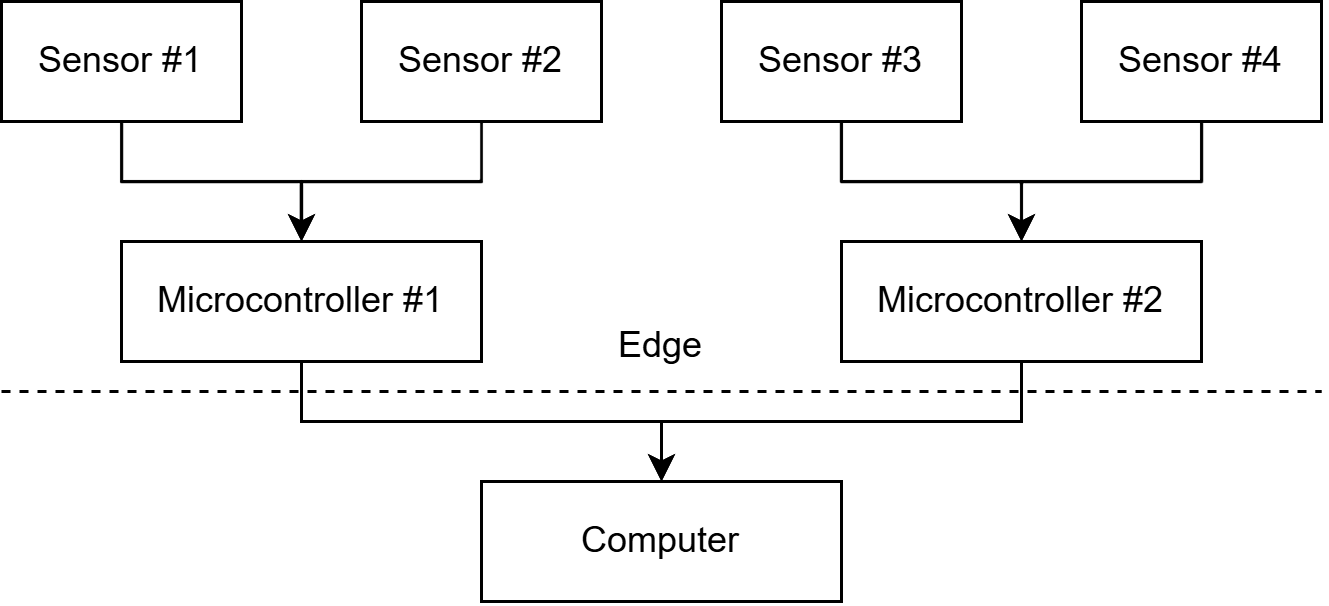
\includegraphics[width=0.7\linewidth]{img/hl_overview}
			\caption{High-level overview of the physical system}
			\label{fig:hloverview}
		\end{figure}
	
	\section{Software}
	On the other hand, Figure \ref{fig:swoverview} shows how the data flows between all subsystems. Images are generated by the sensors and are then fed to the microcontrollers for pre-processing, after which the model uses them to gauge what crops are present in the image and if they are afflicted by disease, nutrient deficiency or another visible predicament.
	
		\begin{figure}[ht]
			\centering
			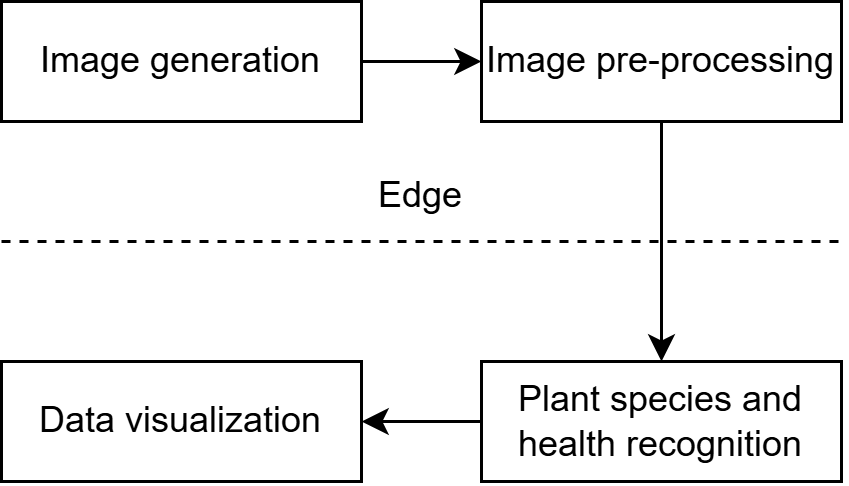
\includegraphics[width=0.7\linewidth]{img/sw_overview}
			\caption{High-level overview of system data flow}
			\label{fig:swoverview}
		\end{figure}
	
	\section{User interface}
	The main goal of the user interface design is to be simple and intuitive. The \gls{gui} application should display the number of scanned images and, for every abnormal or unhealthy plant, it should display the cause. Additionally, images should be associated with a geographical location in order to locate and, if possible, treat the plant. Figure \ref{fig:gui} shows what the design might look like.
	
	\begin{figure}[ht]
		\centering
		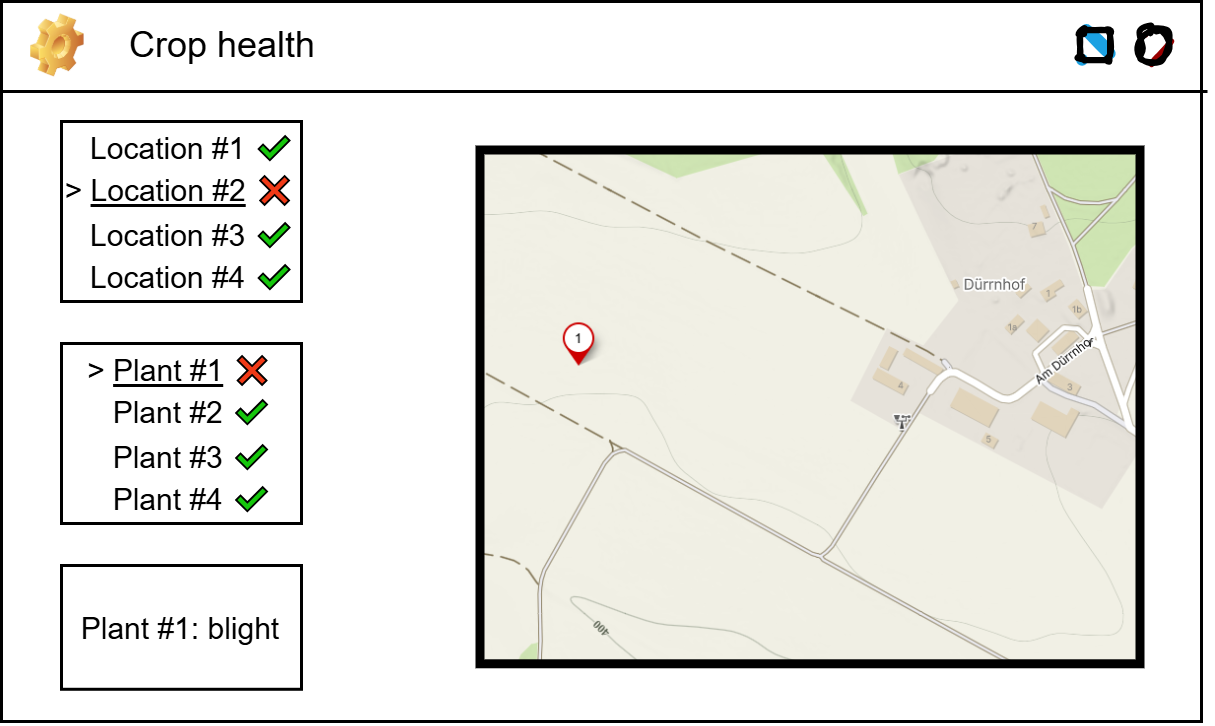
\includegraphics[width=0.7\linewidth]{img/gui}
		\caption{Sample \gls{gui} design}
		\label{fig:gui}
	\end{figure}
	
	\chapter{Further development}

	There are several directions that development can take, with the largest factor in future plans being whether to focus on expanding and scaling the hardware platform or optimizing the software suite.
	
	If software takes precedence in the future, the most important functionality expansion is to build support for detecting different types of crop diseases. Ideally, the system would be able to determine if a plant is diseased or if it is lacking soil nutrients or water. Various small improvements should also be made to the \gls{gui} to accommodate any future updates and provide a more meaningful insight to the user. Image pre-processing can also be tuned to improve performance.
	
	For a holistic approach to system improvement, the hardware platform on which the software operates should also be considered. Initial proposals for the system design propose both \glspl{sbc} and microcontrollers, but focus on the latter. The system was originally designed to execute functionality with lower computing cost at the edge, due to the nature of microcontrollers. By switching to \glspl{sbc}, which have much more computing power, significantly more workload can be delegated to the edge. The ultimate goal with a \gls{sbc}-centered would be to do host all operations on the edge, including the \gls{cnn}-based plant and disease recognition. A question that always looms large with any system of this kind is how can the storage be handled? The semi-centralized model shown in Chapter \ref{chap:project_architecture} has less storage issues, but migrating to the \gls{sbc}-based model will exacerbate them, so different storage solutions will need to be explored.
	
	\chapter{Literature review}	
	Agriculture is central to the forming and maintenance of society, which is why it is not surprising that there is a plethora of papers on how it can be modernized. 
	
	The central theme of this project is the application of computer vision to plant health monitoring. The suitability of \glspl{cnn} models for the use case is clearly demonstrated by Demilie \cite{demilie2024plant} and Tiwari et al \cite{tiwari2021dense}, who also provide an overview of the state of the art. Additionally, Thakur et al \cite{thakur2023vgg} have explored \gls{cnn} methods for plant monitoring in particular, as well as image pre-processing techniques, and their findings are applicable to this project. Agarwal et al \cite{agarwal2020development} have also proposed a similarly lightweight model, though theirs has a more narrow focus. Still, it performs well and its development can inform the implementation of this project. 
	
	Though popular in the world of technology, edge computing has yet to be widely adopted by agriculture. In fact, the application of edge computing models is still understudied and practical implementations are few. For example, Gong et al \cite{gong2025edge} present a very theoretical work. Despite that, it outlines important structural considerations for future implementation. A more practical approach can be seen in this paper by Kim et al \cite{kim2025real}, who have worked with existing models and proprietary edge computing platforms to demonstrate two \gls{poc} solution. While the goal of their research does not align with this project, their methodology and results will have bearing on the execution of this project.
	
	\printglossary[type=\acronymtype]
	\printbibliography
	
\end{document}